% CREATED BY DAVID FRISK, 2016
\chapter{Results}
Lorem ipsum dolor sit amet, consectetur adipisicing elit, sed do eiusmod tempor incididunt ut labore et dolore magna aliqua. Ut enim ad minim veniam, quis nostrud exercitation ullamco laboris nisi ut aliquip ex ea commodo consequat. Duis aute irure dolor in reprehenderit in voluptate velit esse cillum dolore eu fugiat nulla pariatur. Excepteur sint occaecat cupidatat non proident, sunt in culpa qui officia deserunt mollit anim id est laborum.

\section{Sample case. Kleinmaterial: Nätverk}
Each teaching material tested has a different story to tell. Keep in mind that some of the content of the steps below are common to all teaching materials tested and some are original to the particular teaching material.

\subsection{The preexisting work}
The sample teaching material...
\begin{description}
    \item $\bullet$ ...had been produced by a team, consisting of a handful of teachers, a subject expert and a Klein-representative.
    \item $\bullet$ ...was published on Kleindagarna's website.
\end{description}

\subsection{Usability test I}
This first usability test was performed by one of the authors of this report on the other author, primarily to identify what to take into account for future usability testing and to identify the possibility of improving the usability testing methodology. The methodology consisted of a document on a computer including a table made to be filled with personal information and a list of keywords and questions (manuscript) inspired by the usability test script created by Steve Krug. Results from this test included:
\begin{description}
    \item $\bullet$
    \item $\bullet$
\end{description}
\subsection{Revision of methodology}
After usability testing the teaching material, the authors identified that there was very limited information presented in the list of teaching materials on Kleindagarna's website. This made it difficult for the curious to know if the material was suitable for them. Because of that, a new list of teaching materials was compiled. This consisted of information not just what the subject of the material was, but also for what grade it was suited and a more detailed description of the teaching material.\\
Another feature discussed after the usability test was whether teaching materials should be revised as a document solely intended as a foundation that a teacher later could build a lesson around or if revisions instead should design the teaching materials as ready-made presentations, giving the teacher a choice to use it as-is, altering it or just using it as inspiration. The discussion culminated in the decision to decide on a case-by-case basis, considering factors such as results from usability tests, perceived intent of original creators and what form would be most suited to the particular teaching material.
\subsection{Usability test II}
The same revision was tested again. The test subject this time was a Klein-representative that had been involved in the creation of the original teaching material. Testing teaching materials on a subject that wasn't a teacher in upper secondary school or a teacher student aiming to teach at upper-middle school wasn't the norm. One purpose of this was to analyze how rewarding usability testing non-intended subject could be. The test subject is also teaching mathematics on an upper secondary school level, but to post upper secondary school students (although the pace of the courses comparably higher than in upper-middle-school). Results from this test included:
\begin{description}
    \item $\bullet$
    \item $\bullet$
\end{description}
\subsection{Revision of teaching material}
From the data collected, the following revisions were made:
\begin{description}
    \item $\bullet$
    \item $\bullet$
\end{description}
\subsection{What was learned from this case?}
From this particular case, the following knowledge was obtained:
\begin{description}
    \item $\bullet$
    \item $\bullet$
\end{description}

\section{The materials list}
\begin{figure}[H]
\centering
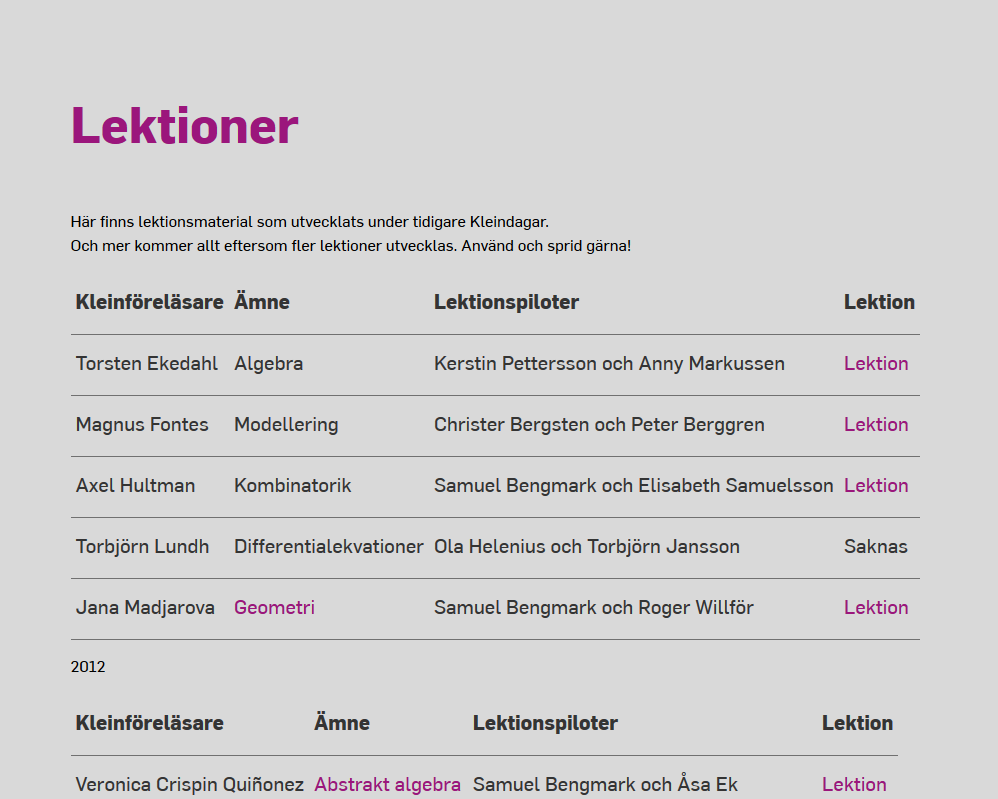
\includegraphics[width=\linewidth]{figure/screenshot_materiallista_kleindagarna.png}
\caption{The original list of materials on Kleindagarna's official website [SOURCE].}
\end{figure}

It is important to note that the design of Kleindagarna's list of materials changed in the middle of the thesis. Most of the information in the list remained the same, but colors and fonts changed. A screenshot of the list before Kleindagarna's change wasn't made and thus the exact changes were lost. The first and second thesis-revisions of the list were made before Kleindagarna made changes to their list.

\begin{figure}[H]
\centering
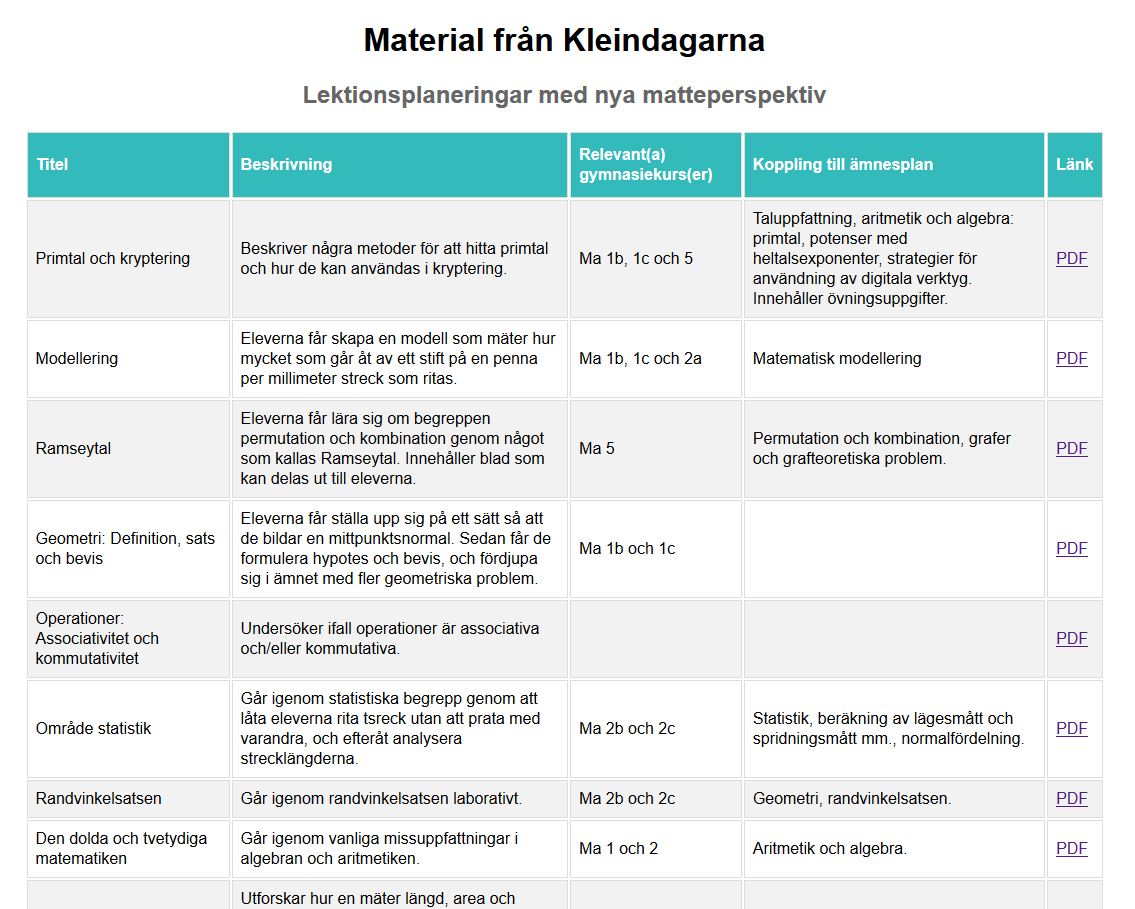
\includegraphics[width=\linewidth]{figure/screenshot_materiallista_revision_2.png}
\caption{The second revision of the list of materials, based on Kleindagarna's original [FIGURE REFERENCE?].}
\end{figure}
